\documentclass{article}
\usepackage{import}

\subimport*{core/included_packages}{included_packages.tex}
\subimport*{core/included_modules}{included_modules.tex}

\setmainlanguage{english}
\setotherlanguage{greek}
\newfontfamily\greekfont{Times New Roman} % or any font that supports Greek


% Macro definition for SunTzuPlaylist
\newtcolorbox{sunztuplaylistbox}[1][]{
  colback=gray!5!white,
  colframe=black!80!white,
  title=#1,
  fonttitle=\bfseries,
  breakable,
  left=1em,
  right=1em,
  top=1em,
  bottom=1em
}

\newcommand{\SunTzuPlaylist}[2]{%
  \begin{sunztuplaylistbox}[#1]
    \begin{enumerate}
      #2
    \end{enumerate}
  \end{sunztuplaylistbox}
}



% Define the tcolorbox environment
\newtcolorbox{psychologysidebarbox}[1][]{
  colback=gray!5!white,
  colframe=black!80!white,
  title=#1,
  fonttitle=\bfseries,
  breakable,
  left=1em,
  right=1em,
  top=1em,
  bottom=1em
}

% Define the PsychologySidebar environment
\newenvironment{PsychologySidebar}[1]
  {\begin{psychologysidebarbox}[#1]}
  {\end{psychologysidebarbox}}
  
  
\begin{document}

  \onehalfspacing
  \setlength{\parskip}{1.5em} 


  %\subimport*{core/included_modules/module/title_page}{title_page.tex}

  \begin{titlepage}
    \centering
  
    {\LARGE\bfseries The Complicity Spiral: How to Make Everyone Dirty So No One Can Cleanly Leave \par}
    \vspace{1em}
    {\large Power, Money, Sex, and How Everyone Gets Used For Something \par}
    {\small Miles A. Head \par}
    
  
    \vfill


  
    \begin{figure}[H]
      \centering
      
      % === First row ===
      \begin{subfigure}[t]{0.45\textwidth}
      \centering
      \begin{tikzpicture}
        \comicpanel{0}{0}
          {Megacorp Dev}
          {Megacorp Exec}
          {\small I spent one month getting access to file a support ticket.}
          {(-0.8,-0.6)}
      \end{tikzpicture}
      \caption*{Enterprise-grade stagnation.}
      \end{subfigure}
      \hfill
      \begin{subfigure}[t]{0.45\textwidth}
      \centering
      \begin{tikzpicture}
        \comicpanel{0}{0}
          {Manager}
          {Startup Intern}
          {\small I deployed to prod from my phone at 3am. It scaled. Probably.}
          {(0.6,-0.6)}
      \end{tikzpicture}
      \caption*{Velocity > supervision.}
      \end{subfigure}
      
      \vspace{1em}
      
      % === Second row ===
      \begin{subfigure}[t]{0.45\textwidth}
      \centering
      \begin{tikzpicture}
        \comicpanel{0}{0}
          {Megacorp HR}
          {Interviewee}
          {\small We offer medical, dental, and diversity training that will make you hate this company.}
          {(-0.6,-0.6)}
      \end{tikzpicture}
      \caption*{The corporate incentive package.}
      \end{subfigure}
      \hfill
      \begin{subfigure}[t]{0.45\textwidth}
      \centering
      \begin{tikzpicture}
        \comicpanel{0}{0}
          {PhD Postgrad}
          {Startup Founder}
          {\small Work for me, and I'll give you \$300k, a fake title, and unlimited cocaine and hookers.}
          {(0.6,-0.6)}
      \end{tikzpicture}
      \caption*{The startup incentive package.}
      \end{subfigure}
      
      \caption*{\textbf{Why the Best Engineers Work at Startups (and Not for You)}}
    \end{figure}
      
  
  \end{titlepage}

  \subimport*{core/included_modules/module/disclaimer}{disclaimer.tex}



  \section*{Foreword}
  
  \bigskip
  
  \textbf{To Whom It May Concern (especially corporate counsel):}
  
  The book you’re about to read is a complete work of fiction.
  
  Any resemblance to actual founders, VCs, consultants, PR flacks, compliance departments, or 
  ``visionary'' platform evangelists is purely coincidental, tragic, and --- frankly --- your own fault 
  for drawing connections where none officially exist.
  
  \textbf{Let me state clearly, for the record, and for the discovery process:}
  This book is officially an imaginary work 
  constructed from (but not limited to) hypothetical observations, apocryphal anecdotes, and several long evenings of 
  bourbon-fueled storytelling in airport lounges.
  \footnote{Portions of this sentence were later redacted in settlement.}

  If any reader, investor, or regulatory agency believes otherwise, I cordially invite you to prove 
  in a court of law that this ``entirely fictitious'' account is, in fact, non-fiction.

  
  If, by some odd twist of fate, you believe that I have violated a non-disclosure agreement, 
  trade secret covenant, or federal gag order, please please please sue me.

  Make your case. Show the world that what I wrote was so accurate --- and so uncomfortably true --- 
  that it could only have come from behind closed doors. That would be, quite honestly, the best press 
  I’ve ever gotten.
  
  \begin{flushright}
    \textit{— Yours in perpetual misalignment,}\\
    \textit{a culturally unretained stakeholder of record}
    \end{flushright}

  \section*{This Is Fiction (Unless It Isn’t): About the Series}

  The book you're reading is part of a larger, ongoing experiment in narrative disclosure.  
  The series is called \textbf{\textit{Startup Sins: Terms and Conditions May Destroy You}}. And yes, 
  the name is a warning.
  
  Each volume offers a different lens into the power structures of modern tech culture. And not the 
  one shown onstage at launch events, but the one muttered over late-night Slack threads, negotiated in 
  hallway whispers, and buried in unread compliance docs.
  
  The stories in this series were not written to expose specific people or companies.  
  They were written to expose the kind of patterns you start to see when pitch decks outnumber 
  product roadmaps, and institutional power hides behind the velvet curtain of founder mythology.
  
  We live in an era where startup culture promises revolution but delivers consolidation.
  Where innovation is just rebranded infrastructure, and where power operates not through violence, 
  but through vocabulary.
  
  In this world:
  
  \begin{itemize}
    \item ``Agility'' means no accountability.
    \item ``Vision'' means vibes with a vest.
    \item ``Transformation'' usually means someone in ops is about to get laid off while marketing posts about empathy.
  \end{itemize}
  
  The motivation for this series was simple:
  Too many people are too fluent in bullshit.
  Too many rooms are filled with brilliant minds saying nothing, wrapped in synergy decks, and 
  rewarded for their ability to confidently explain nothing in five different ways.
  
  Also, I'll be honest about the real spark behind this particular book:
  \textbf{HBO’s \textit{Silicon Valley}}.
  
  I hated that show.
  I did not hate it because it was bad.
  I hated it because it was \textit{too good}.  
  I hated it because it was \textit{too painfully good}. 
  
  I couldn’t get through more than two episodes without pausing to whisper, 
  \textit{``I was in that meeting.''}
  
  It wasn’t funny when it happened to me.
  It was traumatic.
  \textit{How dare they!}
  
  Imagine seeing your worst professional gaslighting repackaged as Emmy-nominated comedy.
  
  Imagine watching your dignity turned into a punchline between commercial breaks.
  
  So this book isn’t revenge.
  It’s just... a counterpunch.
  It is a reminder that if you're going to make jokes about startup hell, the people who 
  actually lived there deserve a little narrative justice.
  
  \begin{quote}
  \textit{I didn’t laugh at that scene because I was under investigation for that exact thing.}\\[1ex]
  \noindent
  \begin{flushright}
  \makebox[0.66\linewidth][r]{%
    \parbox{0.66\linewidth}{\raggedleft
      \small --- Former tech exec,\\ speaking anonymously\\
      (but we both know who you are)}
  }
  \end{flushright}
  \end{quote}

  \section*{Special Thanks (And No, You Can’t Subpoena Gratitude)}

  First, a heartfelt thank you to the usual suspects:  
  friends, colleagues, and collaborators.  

  I want to thank the ghostwriter who swore this wasn't about him.  

  I want to thank the lawyer who proofread this while chain-smoking behind a WeWork.  

  I want to thank the intern who deleted all the Slack threads just in case.

  You know who you are.

  But most importantly — and I say this with deep sincerity and legally non-binding admiration —  
  I’d like to thank all the:
  
  \begin{itemize}
    \item The hookers who took Bitcoin before it was cool. Particularly, that one who may or may not 
    have introduced me to my first investor.
    
    \item The strippers who offered better competitive intel than our strategy team ever did... 
    including that one unforgettable night that may or may not have ended with a pitch deck, a burner phone, 
    and someone's VP of Product in tears.
    
    \item The drug dealers who taught me a lesson no accelerator ever could:  
    that the smartest operators never use their own product.  
    It explaiend why so many corporate executives lose their minds.  
    They believe the pitch deck.  
    And because no one around them is brave (or underpaid enough) to tell them the truth.
    
    \item The unicorns (both startup and lifestyle varieties) who taught me everything I know about scalable performance under high-pressure conditions.
    
    \item The disgruntled employees who quietly forwarded the receipts... some of whom may or may not still have admin privileges.
    
    \item The screwed-over founders who finally admitted that NDAs are just trauma blankets with timestamps... and let me quote them anonymously anyway.

    \item The VC partners who explained term sheets like they were bedtime stories...  
    then turned around and ghosted us faster than a demo day sandwich tray.  
    Special thanks to the one who said, ``We believe in your vision,''
    right before backing our direct competitor's bridge round.
  \end{itemize}
  
  If you recognized yourself in any of the pages that follow, I assure you:  
  \textbf{that’s purely coincidental}... and extremely well-earned.

  Without your whispered stories, midnight vent sessions, encrypted voice notes, and blackout brunches,  
  this book would’ve been a lot less interesting... and a lot more defensible in court.

  To every founder who got ghosted by their Series B... 
  
  And to every ops lead who watched their equity vanish in a “reorg,”... 

  And to every compliance officer who accidentally joined a cult... 

  \textit{This one’s for you.}

  You were the real pitch deck.  

  You were the real due diligence.  

  You were the real risk disclosure buried in the footnotes no one ever reads.

  \begin{flushright}
  \textit{— With gratitude and probable deniability,}\\
  \textit{The author}
  \end{flushright}

  
  
  


  \tableofcontents

  \newpage


  \subimport*{core/part/1_introduction}{introduction.tex}
  \subimport*{core/part/2_mathematical_structures}{mathematical_structures.tex}
  \subimport*{core/part/3_mathematical_analysis}{mathematical_analysis.tex}
  \subimport*{core/part/4_mathematical_uncertainty}{mathematical_uncertainty.tex}
  \subimport*{core/part/5_mathematical_computation}{mathematical_computation.tex}
  \subimport*{core/part/6_mathematical_foundations}{mathematical_foundations.tex}
  \subimport*{core/part/7_ml_use_case}{ml_use_case.tex}
  \subimport*{core/part/8_ml_reality}{ml_reality.tex}
  \subimport*{core/part/9_consulting_strategies}{consulting_strategies.tex}

\end{document}
